\documentclass[problem]{mcs}

\begin{pcomments}
  \pcomment{CP_build_MSTs}
  \pcomment{ARM 10/27/11}
  \pcomment{F11.cp9m, F15.cp8w}
  \pcomment{figure addded, revised ARM 10/21/15}
\end{pcomments}

\pkeywords{
 spanning_tree
 weighted_tree
 minimum_weight
 MST
}

%%%%%%%%%%%%%%%%%%%%%%%%%%%%%%%%%%%%%%%%%%%%%%%%%%%%%%%%%%%%%%%%%%%%%
% Problem starts here
%%%%%%%%%%%%%%%%%%%%%%%%%%%%%%%%%%%%%%%%%%%%%%%%%%%%%%%%%%%%%%%%%%%%%

\begin{problem}
Let $G$ be the $4 \times 4$ grid with vertical and horizontal edges
between neighboring vertices and edge weights as shown in
Figure~\ref{fig:4x4}.

In this problem you will practice some of the ways to build
minimum-weight spanning trees.  For each part, list the edge weights
in the order in which the edges with those weights were chosen by the
given rules.

\iffalse
  Formally,
\[
\vertices{G} = [0,3]^2 \eqdef \set{(k,j) \suchthat 0 \leq k,j \leq 3}.
\]
Letting $h_{i,j}$ be the horizontal edge $\edge{(i,j)}{(i+1,j)}$ and
$v_{j,i}$ be the vertical edge $\edge{(j,i)}{(j,i+1)}$ for $i\in[0,2],
j \in [0,3]$, the weights of these edges are
\begin{align*}
w(h_{i,j}) & \eqdef  \frac{4i+j}{100},\\
w(v_{j,i}) & \eqdef 1+\frac{i+4j}{100}.
\end{align*}
\fi

%\begin{center}
\begin{figure}[h]
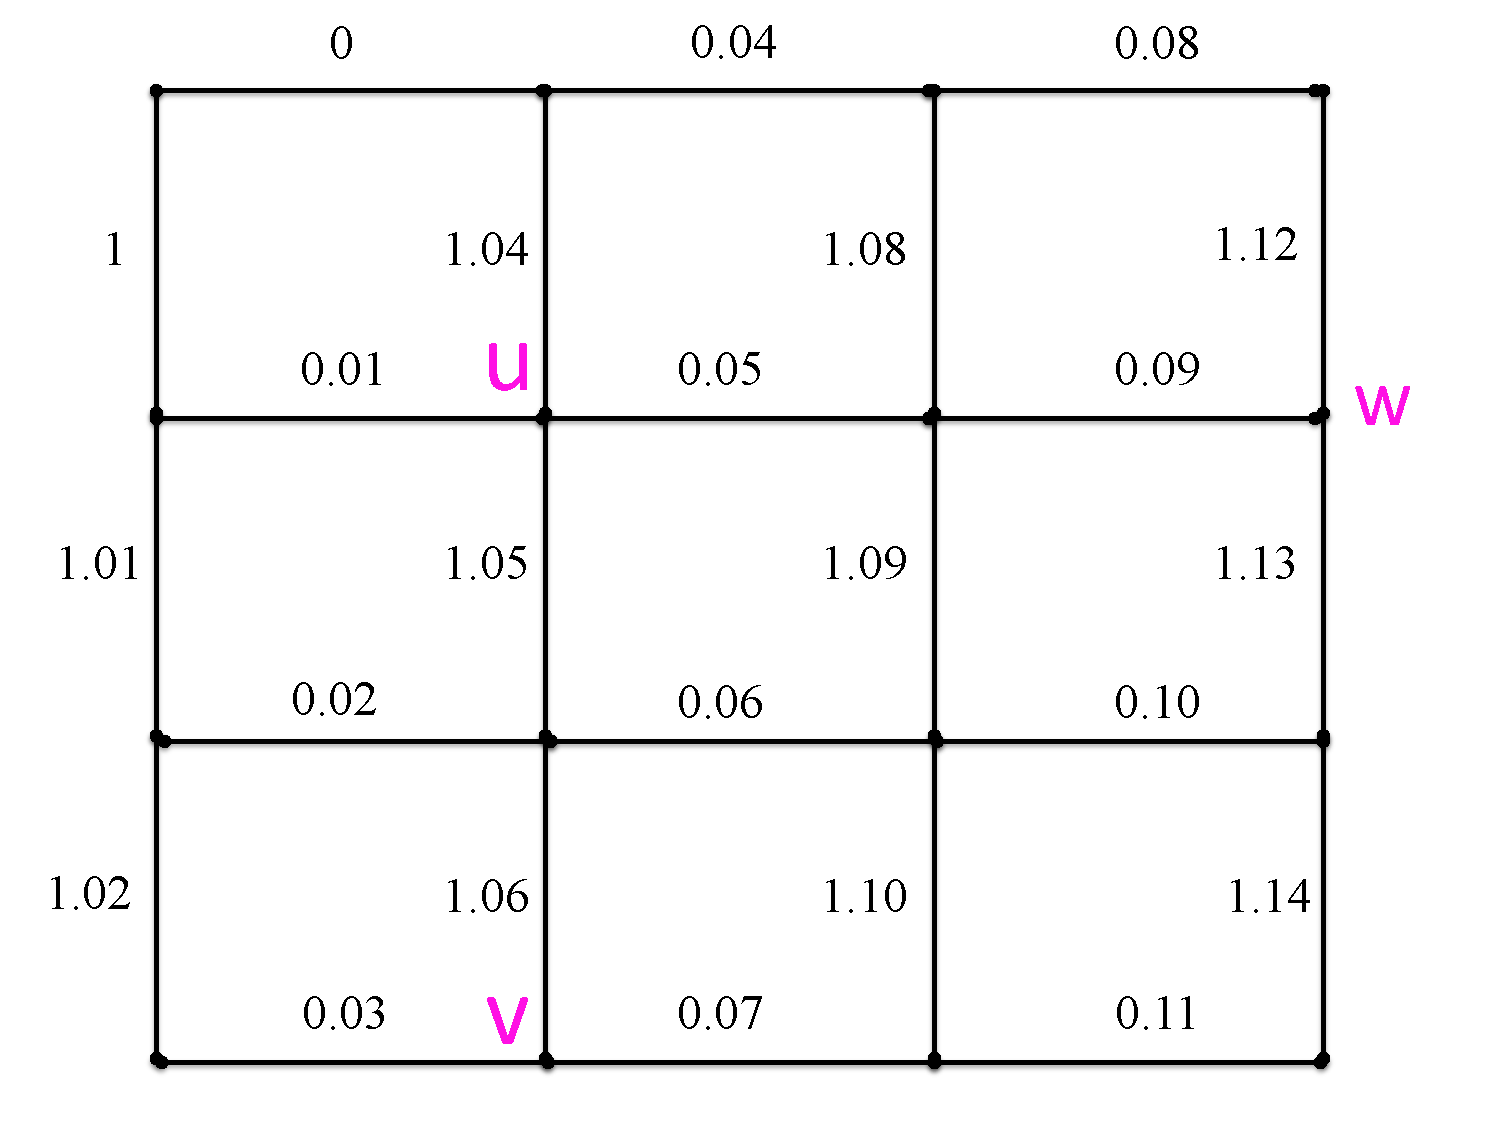
\includegraphics[height=4in]{4x4-array.pdf}
\caption{The 4x4 array graph $G$}
\label{fig:4x4}
\end{figure}
%\end{center}

\bparts

\ppart Construct a minimum weight spanning tree (MST) for $G$ by
initially selecting the minimum weight edge, and then successively
selecting the minimum weight edge that does not create a cycle with
the previously selected edges.  Stop when the selected edges form a
spanning tree of $G$.  (This is Kruskal's MST algorithm.)

For any step in Kruskal's procedure, describe a black-white coloring
of the graph components so that the edge Kruskal chooses is the
minimum weight ``gray edge'' according to
Lemma~\bref{lem:enough-gray}.

\begin{staffnotes}
Students are often unclear about the ``gray edge'' rule.  If the
problem drags, coaches can explain how the rule applies here and in
the next part, and let students work it out for the last part.
\end{staffnotes}

\begin{solution}
\[
0,\ .01,\ .02,\ .03,\ .04,\ .05,\ .06,\ .07,\ .08,\ .09,\ .10,\ .11,\ 1,\ 1.01,\ 1.02
\]

From the text~\bref{alg:MST2}: ``An edge does not create a cycle iff
it connects different components.  The edge chosen by Kruskal's
algorithm will become the minimum weight gray edge of a black-white
coloring when the components it connects are assigned different
colors.''

To explain more fully, suppose Kruskal's procedure choses some
particular edge $e$ at some stage.  This means that when $e$ is
chosen, there is some spanning forest $F$ defined by edges chosen at
previous stages, and among all the remaining edges that do not create
a cycle when added to $F$, the lowest weight edge is $e$.  We want to
show that $e$ can be a minimum weight gray edge in some black-white
coloring.  To do this, note that since $e$ does not create a cycle
when added to $F$, it must connect two distinct components of $F$.
Color one of these components black and color all the other vertices
white.  Any gray edge in this coloring connects two different
components of $F$, and so none of these gray edges creates a cycle
when added to $F$.  Since $e$ is the minimum weight edge that does not
create a cycle, it is certainly minimum weight among these gray edges.
\end{solution}

\ppart Grow an MST for $G$ by starting with the tree consisting of the
single vertex $u$ and then successively adding the minimum weight edge
with exactly one endpoint in the tree.  Stop when the tree spans $G$.
(This is Prim's MST algorithm.)

For any step in Prim's procedure, describe a black-white coloring of
the graph components so that the edge Prim chooses is the minimum
weight ``gray edge''\inbook{according to
  Lemma~\bref{lem:enough-gray}}.

\begin{solution}

\begin{staffnotes}
Old soln:
\[
h_{0,2}h_{1,2}h_{2,2}v_{0,1}h_{0,1}h_{1,1}h_{2,1}v_{0,0}h_{0,0}h_{1,0}h_{2,0}v_{0,2}h_{0,3}h_{1,3}h_{2,3}
\]
\end{staffnotes}

\[
.01,\ .05,\ .09,\ 1,\ 0,\ .04,\ .08,\ 1.01,\ .02,\ .06,\ .10,\ 1.02,\ .03,\ .07,\ .11
\]

From the text~\bref{alg:MST1}: ``This is the algorithm that comes from
coloring the growing tree black and all the vertices not in the tree
white.  Then the gray edges are the ones with exactly one endpoint in
the tree.''

\end{solution}

\ppart The 6.042 ``parallel'' MST algorithm can grow an MST for $G$ by
starting with the upper left corner vertex along with the vertices
labelled $v$ and $w$.  Regard each of the three vertices as one-vertex
trees.  Successively add, for each tree in parallel, the
minimum-weight edge among the edges with exactly one endpoint in the
tree.  Stop working on a tree when there is an edge connecting it to
another tree.  Continue until there are no more eligible trees---that
is, each tree is connected by an edge to another tree---then go back
to applying the general gray-edge method until the parallel trees
merge to form a spanning tree of $G$.

\begin{solution}
Done in parallel:
\begin{align*}
\text{ul} & :\  0,\ .04,\ .08, \text{(no more eligible edges)}\\
       v  & :\ .03,\ .07,\ 0.11, 1.02, 0.02, 0.06, 0.01\\
       w  & :\ .09,\ .05,\ .01, \text{(no more eligible edges)}\\
       \text{remaining gray edges} & :\ 1, 1.01
\end{align*}

\end{solution}

\ppart Verify that you got the same MST each time as \inbook{promised by 
Corollary~\bref{cor:uniqMST}}\inhandout{explained in the text}.

\begin{solution}
They are the same---if no mistake was made.
\end{solution}

\eparts

\end{problem}

%%%%%%%%%%%%%%%%%%%%%%%%%%%%%%%%%%%%%%%%%%%%%%%%%%%%%%%%%%%%%%%%%%%%%
% Problem ends here
%%%%%%%%%%%%%%%%%%%%%%%%%%%%%%%%%%%%%%%%%%%%%%%%%%%%%%%%%%%%%%%%%%%%%

\endinput
